\documentclass[a4paper,12pt]{article}
\usepackage[utf8]{inputenc}
\usepackage{graphicx}
\usepackage{tikz}
\usetikzlibrary{shapes.geometric, arrows}
\usepackage{xcolor}
\usepackage{listings}
\usepackage{ragged2e}
\usepackage{geometry}
\usepackage{amssymb}


\begin{document}
\begin{center}
\textbf{Assignment-8 \\
\vspace{5mm}
ELP - 718 Telecom Software Laboratory \\
\vspace{2mm}
Shivaji Roy \\
2018JTM2002 \\
2018-2020} \\
\vspace{10mm}
A report presented for the assignment-8 \\
\vspace{30mm}

\includegraphics[scale=0.5]{iitlogo} \\
\vspace{10mm}
Bharti School Of \\
Telecommunication Technology and Management \\
IIT Delhi \\
India \\
September 27, 2018

\end{center}
\newpage
\tableofcontents
\newpage
\section{Objective}
To develop our logical skills to solve the given problem with the help of basic python syntax.
\section{Problem Statement 1}
IIT Delhi, has just got the strongest computer. The professors in charge wants to check the computational capacity of the computer. So, they decided to create the problem which is to be given as an assignment to students. Can you help the professor to check the computation capability of the computer?

A valid cross is defined here as the two regions (horizontal and vertical) of equal lengths crossing over each other. These lengths must be odd, and the middle cell of its horizontal region must cross the middle cell of its vertical region.

Find the two largest valid crosses that can be drawn on smart cells in the grid, and return two integers denoting the dimension of the each of the two largest valid crosses. In the above diagrams, our largest crosses have dimension of 1,  5 and 9 respectively .

Note: The two crosses cannot overlap, and the dimensions of each of the valid crosses should be maximal.



\subsection*{Constraints}
\begin{itemize}
\item $2 \leqslant n \leqslant 105$
\item $2 \leqslant m \leqslant 105$

\end{itemize}

\subsection{Program structure}


\tikzstyle{startstop} = [rectangle, rounded corners, minimum width=3cm, minimum height=1cm,text centered, draw=black, ]

\tikzstyle{io} = [trapezium, trapezium left angle=70, trapezium right angle=110, minimum width=3cm, minimum height=1cm, text centered, draw=black, ]

\tikzstyle{process} = [rectangle, minimum width=3cm, minimum height=1cm, text centered, draw=black, ]

\tikzstyle{decision} = [diamond, minimum width=3cm, minimum height=1cm, text centered, draw=black,]


\tikzstyle{arrow} = [thick,->,>=stealth]



\begin{tikzpicture}[node distance=2.5cm]

\node (start) [startstop] {Start};
\node (in1) [io, below of=start] {values of rows an columns are made input from the user};
\node (pro1) [process, below of=in1] {scanning};

\node (pro2a) [process, below of=pro1] {using loops and determining the pattern};

\node (stop) [startstop,below of=pro2a] {Stop};

\draw [arrow] (start) -- (in1);
\draw [arrow] (in1) -- (pro1);
\draw [arrow] (pro1) -- (pro2a);

\draw [arrow] (pro2a) -- (stop);
\end{tikzpicture}


\subsection{Input and Output format}
\begin{itemize}
\item \textbf{Input format} \\
The first line contains two space-separated integers,  n and m. 
Each of the next  lines n contains a string of  m characters where each character is either S (Smart) or D (Dull). These strings represent the rows of the grid. If the jth character in the ith  line is S, then  (i,j) is a  cell smart. Otherwise it's a  dull cell..
\item \textbf{Output format}\\
Find two valid crosses that can be drawn on smart cell of the grid, and return the dimension of both the crosses in the reverse sorted order(i.e. First Dimension should be the larger one and other should be smaller one).\\
\end{itemize}
\subsection{Test Cases}
\textbf{Sample Input1}\\
5 6 \\
SSSSSS\\
SDDDSD\\
SSSSSS\\
SSDDSD\\
SSSSSS\\
\textbf{Sample Output0} \\
5 1\\
\textbf{Sample Ouput1} \\
6 6 \\
DSDDSD\\
SSSSSS\\
DSDDSD\\
SSSSSS\\
DSDDSD\\
DSDDSD\\
\textbf{Sample Intput2} \\
5 9 \\
SSSSDSDDD\\
DDSDDDDDD\\
SSSSSDDDD\\
DDSDDSDDD\\
DSSSDDDDD\\

\textbf{Sample Output2} \\
9 1



\subsection{Screenshots}

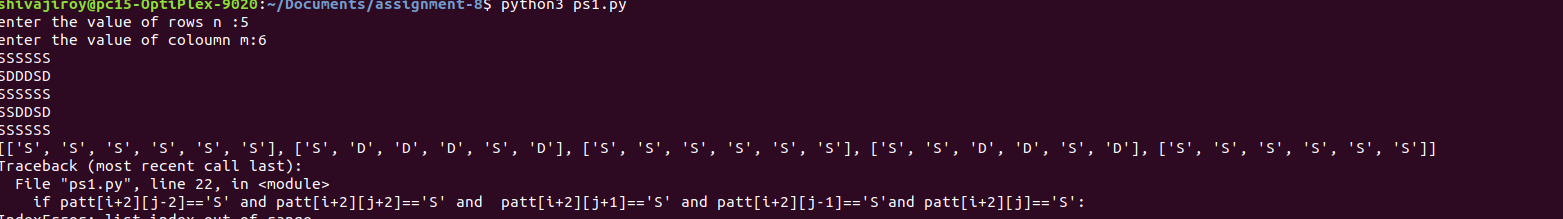
\includegraphics[scale=0.35]{Screenshot1.png}

\section{Problem Statement 2}
\subsection{Problem Statement}
After, getting mix results of valid crosses, professors decided to test the computation abilities on one more problem. This time professors wanted to test the decryption capabilities of the computer.
Encryption of  a message requires three keys, k1, k2, and k3. The 26 letters of English and underscore are divided in three groups,  [a-i] form one group, [j-r] a second group, and everything else ([s-z] and underscore) the third group. Within each group the letters are rotated left by ki positions in the message. Each group is rotated independently of the other two. Decrypting the message means doing a right rotation by ki positions within each group.



\subsection{Input Output Format}
\begin{itemize}
\item \textbf{Input format} \\
All input strings comprises of only lowercase English alphabets and underscores(\textunderscore).\\
\item \textbf{Output format}\\
For each encrypted message, the output is a single line containing the decrypted string. \\
\item \textbf{Constraints} \\
\begin{itemize}
\item $1 \leqslant length of string \leqslant 150$
\item $1 \leqslant ki \leqslant 150(i=1,2,3)$
\end{itemize}
\end{itemize}

\subsection{Test Case}
Sample Input:  2 3 4\\
			   dikhtkor\textunderscore ey\textunderscore tec\textunderscore ocsusrsw\textunderscore ehas\textunderscore \\

Sample Output:  hardworkis\textunderscore the\textunderscore key\textunderscore to\textunderscore success

\subsection{Difficulties/Isseus Faced}
\begin{itemize}
\item Error in code compiling.
\item Error while giving inputs through Terminal.
\end{itemize}
\subsection{Screenshots}

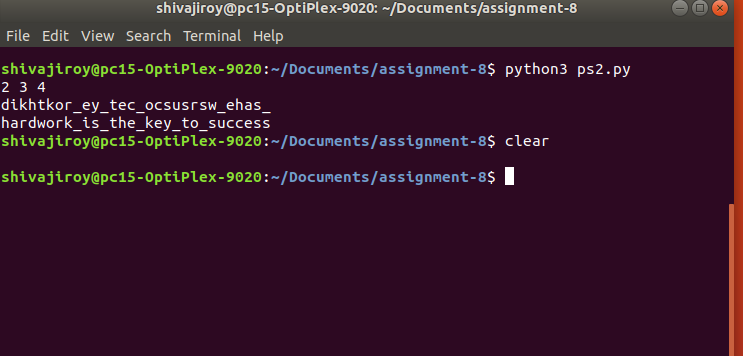
\includegraphics[scale=0.35]{Screenshot2.png}


\section{Appendix}
\subsection{Appendix-A : code for ps1}
\definecolor{mGreen}{rgb}{0,0.6,0}
\definecolor{mGray}{rgb}{0.5,0.5,0.5}
\definecolor{mPurple}{rgb}{0.58,0,0.82}
\definecolor{backgroundColour}{rgb}{0.95,0.95,0.92}

\lstdefinestyle{CStyle}{
    backgroundcolor=\color{backgroundColour},   
    commentstyle=\color{mGreen},
    keywordstyle=\color{magenta},
    numberstyle=\tiny\color{mGray},
    stringstyle=\color{mPurple},
    basicstyle=\footnotesize,
    breakatwhitespace=false,         
    breaklines=true,                 
    captionpos=b,                    
    keepspaces=true,                 
    numbers=left,                    
    numbersep=5pt,                  
    showspaces=false,                
    showstringspaces=false,
    showtabs=false,                  
    tabsize=2,
    language=C
}




\begin{lstlisting}[style=CStyle]
n=int(input("enter the value of rows n :"))
m=int(input("enter the value of coloumn m:"))
patt = []

#creating a array to take the inputs
for i in range(n):
        t = list(input())
        patt = patt + [t]
print(patt)

#running a loop to compare elements
for i in range(n):
        for j in range(m):
                #print(i,j,patt[i][j])

                if patt[i][j]=='S'and patt[i][j+1]=='S' and patt[i][j-1]=='S': # comparision of characters for finding a pattern of 9 S
                        if patt[i+1][j]=='S'and patt[i+1][j-1]=='D' and patt[i+1][j+1]=='D': #comparision of next column to find the pattern
                                if patt[i+2][j-2]=='S' and patt[i+2][j+2]=='S' and  patt[i+2][j+1]=='S' and patt[i+2][j-1]=='S'and patt[i+2][j]=='S': #comparision in the next row and about the same column against its previous and next column 
                                        if patt[i+3][j]=='S'and patt[i+3][j-1]=='D' and patt[i+3][j+1]=='D':#moving to next row and trying to correlate the pattern 
                                                if patt[i+4][j]=='S'and patt[i+4][j+1]=='S' and patt[i+4][j-1]=='S':   
                                                        print("9")

                elif patt[i][j]=='S' and patt[i][j-1]=='D' and patt[i][j+1]=='D' and i<=n-1 : #similarly trying to correlate the pattern regarding 5 S
                        if patt[i+1][j]=='S' and patt[i+1][j+1]=='S' and patt[i+1][j-1]=='S':
                                if patt[i+2][j]=='S' and patt[i][j-1]=='D'and patt[i][j+1]=='D':
                                                print("5")
                elif patt[i][j]=='S' and patt[i][j-1]=='D' and patt[i][j+1]=='D' and i<=n-1 :# similarly trying tyo correlate the pattern regarding 1 S
                        if patt[i+1][j]=='D'and patt[i+1][j-1]=='D' and patt[i+1][j+1]=='D':
                                if patt[i+2][j]=='D'and patt[i+2][j-1]=='D' and patt[i+2][j+1]=='D':
                                        print("1")
\end{lstlisting}

\newpage
\subsection{Appendix-B : code for ps2}
\definecolor{mGreen}{rgb}{0,0.6,0}
\definecolor{mGray}{rgb}{0.5,0.5,0.5}
\definecolor{mPurple}{rgb}{0.58,0,0.82}
\definecolor{backgroundColour}{rgb}{0.95,0.95,0.92}

\lstdefinestyle{CStyle}{
    backgroundcolor=\color{backgroundColour},   
    commentstyle=\color{mGreen},
    keywordstyle=\color{magenta},
    numberstyle=\tiny\color{mGray},
    stringstyle=\color{mPurple},
    basicstyle=\footnotesize,
    breakatwhitespace=false,         
    breaklines=true,                 
    captionpos=b,                    
    keepspaces=true,                 
    numbers=left,                    
    numbersep=5pt,                  
    showspaces=false,                
    showstringspaces=false,
    showtabs=false,                  
    tabsize=2,
    language=C
}




\begin{lstlisting}[style=CStyle]
###### this is the second .py file ###########

####### write your code here ##########
#rotate function
def rotate(lst,x):
    copy = list(lst)
    for i in range(len(lst)):
        if x<0:
            lst[i+x] = copy[i]
        else:
            lst[i] = copy[i-x]


#Create 3 groups
a1="abcdefghi"
a2="jklmnopqr"
a3="stuvwxyz_"

b1 =[]
b2 =[]
b3 =[]
i1=[]
i2=[]
i3=[]

#get key vakue from user
k1,k2,k3 = list(map(int,input().split()))

#get string
msg = input()
msg_list = list(msg)
#print(msg_list)

#now compair g1 in string and copy similaar char into s1
for i in range(0,len(msg)):
	if msg_list[i] in a1:
		b1.append(msg_list[i])
		i1.append(i)
		
	elif msg_list[i] in a2:
	    b2.append(msg_list[i])
	    i2.append(i)
	elif msg_list[i] in a3:
	    b3.append(msg_list[i]) 
	    i3.append(i)



#rotate b1,b2,b3
rotate(b1,k1)
rotate(b2,k2)
rotate(b3,k3)



#get decrypted msg
p=q=r=0
for i in range(0,len(msg)+1):
	if i in i1:
		msg_list[i]=b1[p]
		p+=1
	elif i in index2:
		msg_list[i]=b2[q]
		q+=1
	elif i in index3:
		msg_list[i]=b3[r]
		r+=1	

#print(msg_list)

for i in msg_list[:]:
	print (i, end ='')

print("")
\end{lstlisting}

\nocite{*}
\bibliographystyle{plain}
\bibliography{assign8.bib}
\end{document}